\documentclass[]{report}

\voffset=-1.5cm
\oddsidemargin=0.0cm
\textwidth = 480pt

\usepackage{framed}
\usepackage{subfiles}
\usepackage{graphics}
\usepackage{newlfont}
\usepackage{eurosym}
\usepackage{amsmath,amsthm,amsfonts}
\usepackage{amsmath}
\usepackage{color}
\usepackage{amssymb}
\usepackage{multicol}
\usepackage[dvipsnames]{xcolor}
\usepackage{graphicx}
\begin{document}

\section{Summary of Normal Distribution}



\begin{framed}
	\begin{itemize}
			\item The Standardisation Formula
			
			\[P(X \leq Xo) = P(Z \leq Zo)	  \]  
			
			when   \[Zo=\frac{Xo- \mu}{\sigma}\]
		\item The Complement Rule
		\begin{equation}
		P(Z \leq z_o) = 1 - P(Z \geq z_o)
		\end{equation}
		\item The Symmetry Rule
		\begin{equation}
		P(Z \leq -z_o) = P(Z \geq z_o)
		\end{equation}
		\item The Interval Rule.
		Where $L$ and $U$ are the lower and upper bounds of an interval.
		\begin{equation}
		P(L \leq Z \leq U) = P(Z \geq L) -  P(Z \geq U)
		\end{equation}
		
	\end{itemize}
\end{framed}
	
\section{Normal Distribution : Arab Horses Worked Example}
The mass of Arab horses is normally distributed with mean 900 lbs and standard deviation of 50lbs.
\begin{itemize}
	
	\item  Calculate the probability that an Arab horse weighs more than 940 lbs.
	\item Calculate the probability than an Arab horse weighs between 880 lbs and 960 lbs.
\end{itemize}

\noindent \textbf{Solution}\\

\begin{itemize}
	\item Let X be mass of Arab horses.
	
	\item We have to find $P(X\leq940)$.            (Remark "equality component" is included as a formality, but it is not important)
	
	
	\item	Find the Z value that corresponds to 940 
	
	\[Zo=\frac{Xo-\mu}{\sigma}= \frac{940 -900}{50}= 0.8\]
	
	\[P(X \leq 940) = P(Z \leq 0.8) \]
	
	
	\item		From Murdoch Barnes tables 3, we find that $P(Z \leq 0.8) = 0.2119$
\end{itemize}





Solution 

\[P ( 880 \leq X \leq 960).\]


What proportion of horses are between 880 lbs and 960 lbs?
\begin{itemize}
	\item Find out the probability of the complement event.
	\item The complement event is the combination of being too high  or too low for this interval.
	
	\item Inside interval $P ( 880 \leq X \leq 960).$
	
	\item Outside interval $P (X \leq 880) + P(X \geq 960)$
	
	\item Complement Rule $P ( 880\leq X \leq 960)  = 1 - [P (X\leq 880) +P(X\geq 960)]$
	
\end{itemize}



Find the probability of being too high?

\[Zo=\frac{Xo-\mu}{\sigma}= \frac{960 -900}{50}= 1.2\]

\[P(X \leq 960) = P(Z \leq 1.2) = 0.1151\]


Find the probability of being too low?
\[Zo= \frac{Xo-\mu}{\sigma}= \frac{880 -900}{50}= -0.4 \]
\[P(X \leq 880) = P(Z \leq -0.4)  \]

%------------------------------------------------------------- %
How to compute $P(Z \leq -0.4)$

Symmetry: 	$P(Z \leq -0.4)$ = $P(Z \geq 0.4)$ = 0.3446


\begin{itemize}
	\item Outside Interval = 0.4596        (0.3446 +  0.1151)
	\item Inside Interval = 0.5404
\end{itemize}



%------------------------------------------------------------- %
What weight is exceeded by 97.5\% of Arab horses?

Find Xo  such that P(XXo) = 0.975

\begin{itemize}
	\item 	P(Z1.96) = 0.025     [From Tables] 
	
	\item	P(Z-1.96) = 0.025  [Symmetry]
	
	\item	P(Z-1.96) = 0.975         
	
	\item	\[-1.96 = \frac{Xo- 900}{50} \]
	
	
	\item	Xo= 802 lbs  [Answer]
\end{itemize}	







%----------------------------------------------------%

\section{Exam Question:MA4413 Autumn 2008 paper}

	
		A model of an on-line computer system gives a mean times to retrieve a record from a direct access storage system device of 200 milliseconds, with a standard deviation of 58 milliseconds. If it can assumed that the retrieval times are normally distributed:
		
		\begin{itemize}
			\item[(i)] What proportion of retrieval times will be greater than 75 milliseconds?
			\item[(ii)] What proportion of retrieval times will be between 150 and 250 milliseconds?
			\item[(iii)] What is the retrieval time below which 10\% of retrieval times will be?
		\end{itemize}
		

	\textbf{Normal Distribution}
	
	\begin{center}
		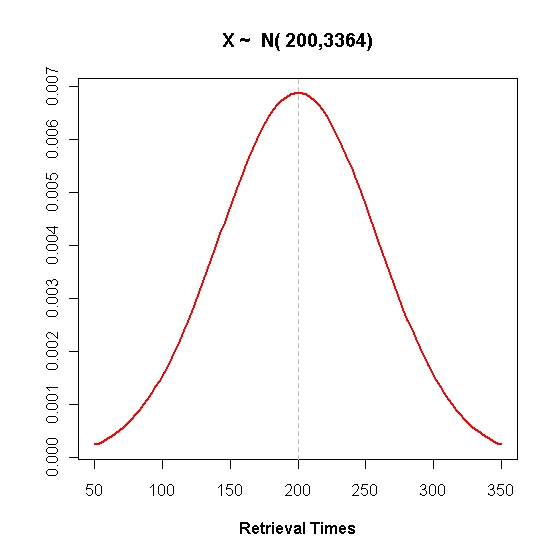
\includegraphics[scale=0.40]{images/5BNormal1}
	\end{center}



	\subsection{Solution to part 1)}
	What proportion of retrieval times will be greater than 75 milliseconds?\\ \bigskip
	
	\begin{itemize}
		\item Let X be the retrieval times, with $X \sim \mbox{N}(200,58^2)$.\\
		\item The first question asks us to find $P( X \geq 75)$. \\
		\item First compute the z score.
		\[ z_o =  {x_o - \mu \over \sigma} = {75 - 200 \over 58}  = -2.15 \]
	\end{itemize}

	
	\textbf{Normal Distribution}
	
	\begin{center}
		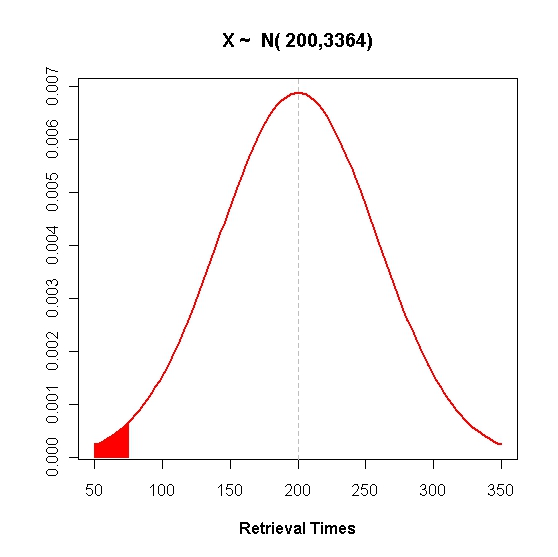
\includegraphics[scale=0.40]{images/5BNormal2}
	\end{center}
	
	In this case, the probability of interest $P(X\geq 75)$, is represented by the white area under the curve.
	
	
	\begin{itemize}
		\item We can say
		\[ P( X \geq 75) = P( Z \geq -2.15)\]
		\item Using symmetry rule and complement rule
		\[ P( Z \geq -2.15) = P( Z \leq 2.15) = 1- P( Z \geq 2.15)\]
		\item From tables $P( Z \geq 2.15) = 0.0158$
		\item Therefore $P( Z \leq 2.15) = 0.9842$
		\item Furthermore $P( X \geq 75) = \boldsymbol{0.9842}$ [Answer].
	\end{itemize}
		

	
	\begin{center}
		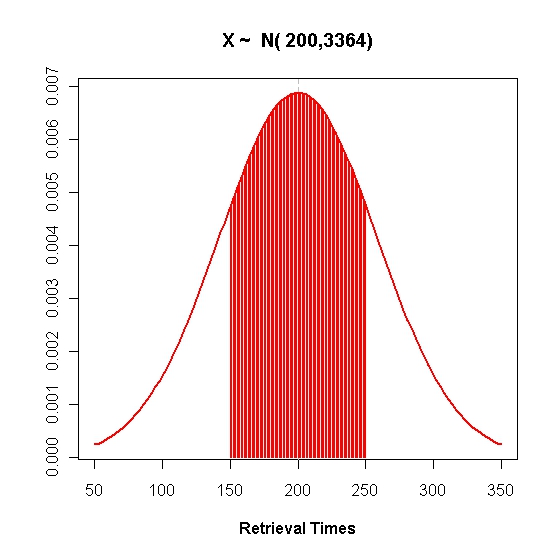
\includegraphics[scale=0.40]{images/5BNormal3}
	\end{center}

	
	\subsection{Solution to part 2)}
	\begin{itemize}
		\item What proportion of retrieval times will be between 150 and 250 milliseconds?
		\item Find $P(150 \leq X \leq 250)$
		\item Use the `Too Low / Too High ' approach.
		\item Too low $P( X \leq 150)$
		\item Too high $P( X \geq 250)$
		\item Find the z-scores for each.
		\[ z_{150} =  {150 - 200 \over 58}  = -0.86 \]
		\[ z_{250} =  {250 - 200 \over 58}  = 0.86 \]
	\end{itemize}

	
	\begin{itemize}
		\item We can now say
		\[ 1. P( X \leq 150) = P( Z \leq -0.86)\]
		\[ 2. P( X \geq 250) = P( Z \geq 0.86)\]
		\item By symmetry rule, $P( Z \leq -0.86) = P( Z \geq 0.86)$
		\[ P( X \leq 150) =  P( X \geq 250) \]
		\item Let's compute $P( X \geq 250)$. Using tables
		\[P( X \geq 250) = P( Z \geq 0.86) = 0.1949 \]
	\end{itemize}


	
	\textbf{Using the Interval Rule}
	\begin{itemize}
		\item Too high: $P( X \geq 250) = 0.1949 $
		\item Too low:  $P( X \leq 150) = 0.1949 $
		\item Probability of being inside interval:
		
		\[ P(150 \leq X \leq 250) = 1- [ P( X \leq 150) + P( X \geq 250)] \]
		
		\item $P(150 \leq X \leq 250) = 1- [ 0.1949 + 0.1949 ] = \boldsymbol{0.6102}$
		
	\end{itemize}	
	
\subsection{Solution to part 3}
	\begin{itemize}
		\item What is the retrieval time below which 10\% of retrieval times will be?
		\item Find $A$ such that $P(X \leq A) = 0.10$.
		\item What z-score would correspond to $A$? Lets call it $z_A$.
		\item $P(Z  \leq z_A) = 0.10$
		\item Remark: $z_A$ could be negative.
		\item Using symmetry $P(Z \geq -z_A) = 0.10$
		\item Remark: $-z_A$ could be positive.
	\end{itemize}


	
\begin{center}
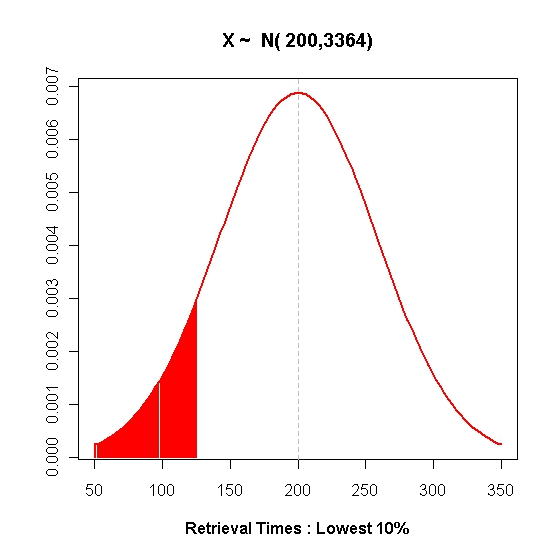
\includegraphics[scale=0.40]{images/5BNormal4}
\end{center}
	

	\begin{itemize}
		\item Use the Murdoch Barnes tables to get an approximate value for $-z_A$.
		\item The nearest value we can get is 1.28. ( $P( Z \geq 1.28) = 0.1003$ ).
		\item If $-z_A = 1.28$, then $z_A=-1.28$
		\item We can now say
		\[ P(X \leq A) = P(Z \leq -1.28) \]
		
	\end{itemize}

	\begin{itemize}
		\item Necessarily $A$ and $Z_A$ are related by the standardization formula
		\item Recall that $\mu = 200$ and $\sigma = 58$.
		\[ -1.28  = {A - 200 \over 58} \]
		\item Re-arranging ( multiply both sides by 58)
		\[ -74.24  = A - 200 \]
		\item Re-arranging again (Add 200 to both sides)
		\[ 125.76 =  A \]
	\end{itemize}
	\begin{itemize}
		\item Now we know the retrieval time below which 10\% of retrieval times will be.
		\item $P(X \leq 125.76) = 0.10$ [Answer].
	\end{itemize}






\subsection{May 2012 Question 4 Normal Distribution / Theory}



%======================================================%
\noindent \textbf{Parameter Values}

Given the parameters of the normal distribution $X$ in the question.
\begin{itemize}
	\item Normal Mean $\mu = 73$ points
	\item Normal Standard Deviation $\sigma = 8$ points
\end{itemize}

\begin{itemize}
	\item $P(X \leq 91)$
	\item $P(65 \leq X \leq 89)$
\end{itemize}
Find the Z score for X = 91.

\[ Z = \frac{x- \mu}{ \sigma} = \frac{91 - 73}{8} =\frac{18}{8} = 2.25\]

Therefore we can say :\\ $P(X \leq 91)$ = $P(Z \leq 2.25)$ \\


From the tables $P(Z \leq 2.25) = 0.9877$
Therefore the probability of getting a grade lower than 91 is 0.9877 (i.e 98.77\%)


What is the probability of getting a score between 65 and 89.
Writing this mathematically:
\[ P(65 \leq X \leq 89) \]

%================================================================%
\begin{itemize}
	\item How many people get a score greater than 89? ($P(X\geq 89)$)
	\item How many people get a score less than 65? ($P(X\leq 65)$)
\end{itemize}

To compute $P(X \geq 89)$ first compute the Z-score.

\[ Z = \frac{x - \mu}{\sigma} = \frac{89 - 73}{8} =\frac{16}{8} = 2 \]

$P(X \geq 89)$ = $P(Z \geq 2)$ = 0.0225.

To compute $P(X \leq 65)$ first compute the Z-score.

\[ Z = \frac{x - \mu}{\sigma} = \frac{65 - 73}{8} =\frac{-8}{8} = -1 \]

$P(X \leq 65)$ = $P(Z \leq -1)$ 

\begin{itemize}
	\item We use the \textbf{symmetry rule}
	\[ P(Z \leq -1) = P(Z \geq +1) \]
	\item so we can say $P(X \leq 65)$ = $P(Z \geq +1)$ 
	\item From the statistical tables $P(Z \geq +1)$ = 0.1583.
\end{itemize}


\subsection{May 2012 Question 5 Normal Distribution }
Given
\begin{itemize}
	\item $X$ is the variable of interest.
	\item Normal Mean $\mu =25.5$ mpg
	\item Normal Standard Deviation $\sigma =4.5$ mpg
\end{itemize}
\begin{itemize}
	\item Find $x$ such that $P(X \geq x) = 0.30$
\end{itemize}
\noindent \textbf{Solution}

From the Standard Normal Tables, find the value of $z$ that would give us
\[ P(Z \geq z) = 0.30 \]
Or if you are using the other type of tables 
\[ P(Z \leq z) = 0.70  \]

%-----------------------------------------------------%

\subsection{May 2013 Question 3 Normal Distributions}

\noindent \textbf{Important Information from the Question}
\begin{itemize}
	\item Normal Mean $\mu$ = 1000 units
	\item Normal Standard Deviation $\sigma$ = 200 units 
\end{itemize}

\noindent \textbf{Objectives}
Compute the following : 
\begin{itemize}
	\item $P(X \geq 1400 )$ More than 1400
	\item $P(X \leq 500)$ Less than 500
\end{itemize}


\noindent \textbf{Part 1 -  More than 1400}

Firstly compute the z score for 1400.

\[ Z_{1400} =  \frac{X - \mu}{\sigma} = \frac{1400 - 1000}{200} = \frac{400}{200} = 2  \]

So the \textbf{Z-score} in this case is 2.

This much we can say
\[P(X \geq 1400) = P(Z \geq 2)\]

$P(Z \geq 2)$ can be determined using statistical tables.
Depending on which statistical tables you are using, you will get one of the following answers. (Note the 
second and third statements are examples of complementary probabilities.)
\begin{itemize}
	\item $P (0 \leq Z \leq 2)$ = 0.4775
	\item $P ( Z \leq 2)$ = 0.9775
	\item $P ( Z \geq 2)$ = 0.0225
\end{itemize}
The last expression is useful here. Recall that $P(X \geq 1400) = P(Z \geq 2)$. Therefore

\[P(X \geq 1400) = 0.0225\]


\subsection*{Objectives}
Compute the following : 
\begin{itemize}
	\item $P(X \geq 1400 )$ More than 1400
	\item $P(X \leq 500)$ Less than 500
\end{itemize}


\noindent \textbf{Part 1 -  More than 1400}

Firstly compute the z score for 1400.

\[ Z_{1400} =  \frac{X - \mu}{\sigma} = \frac{1400 - 1000}{200} = \frac{400}{200} = 2  \]

So the \textbf{Z-score} in this case is 2.

This much we can say
\[P(X \geq 1400) = P(Z \geq 2)\]

$P(Z \geq 2)$ can be determined using statistical tables.
Depending on which statistical tables you are using, you will get one of the following answers. (Note the 
second and third statements are examples of complementary probabilities.)
\begin{itemize}
	\item $P (0 \leq Z \leq 2)$ = 0.4775
	\item $P ( Z \leq 2)$ = 0.9775
	\item $P ( Z \geq 2)$ = 0.0225
\end{itemize}
The last expression is useful here. Recall that $P(X \geq 1400) = P(Z \geq 2)$. Therefore

\[P(X \geq 1400) = 0.0225\]
	

	%-----------------------------------------------------%
	

\section{Normal - example}

In an examination the scores of students who attend schools of type A are
normally distributed about a mean of 55 with a standard deviation of 6. The
scores of students who attend type B schools are normally distributed about a
mean of 60 with a standard deviation of 5.


Which type of school would have a higher proportion of students with marks above 70?

\begin{multicols}{2}
\begin{itemize}
	\item $\mu_A$ = 55
	\item $\sigma_A$ = 8
	
	\item $\mu_B$ = 60
	\item $\sigma_B$ = 5
\end{itemize}
\end{multicols}
We have to fins $P(X_A \geq 70)$
and $P(X_B \geq 70)$.


using the standardisation formula
$Z_A = \frac{70 - 55}{6} = \frac{15}{6} = 2.5 $

$Z_B = \frac{70 - 60}{5} = \frac{10}{5} = 2 $



\newpage

\section{Worked Example 3 - with Solutions}
Assume that the number of weekly study hours for students at a certain university
is approximately normally distributed with a mean of 22 and a standard deviation
of 6.
\begin{enumerate}
	\item Find the probability that a randomly chosen student studies less than 12
	hours.
	\item Estimate the percentage of students that study more than 37 hours.
\end{enumerate}

\textbf{solution}
$X \sim \mathcal(22,6^2)$  ( in form $X \sim \mathcal(\mu,\sigma^2)$\\

Part 1: $P(X \leq 12)$\\


$Z_1 = \frac{12 - 22}{6} = \frac{-10}{6} = -1.66 $\\

Part 2: $P(X \geq 37)$\\

$Z_2 = \frac{37 - 22}{6} = \frac{15}{6} = 2.5 $\\

%----------------------------------------------------%

\section{Worked Example 4 - with Solutions}
The mean is 550kg, with standard deviation 150kg, and we are interested in the area that is greater than 600kg.

\begin{equation}
Z = \frac{ X - \mu }{ \sigma }
\end{equation}

Here X = 600kg,
$\mu$ , the mean = 550kg
$\sigma$, the standard deviation = 150kg
\begin{itemize}
	\item $z = ( 600 - 550 ) / 150$
	\item $z = 50 / 150$
	\item $z = 0.33$
\end{itemize}

Look in the table down the left hand column for z = 0.3, and across under 0.03.
The number in the table is the tail area for z=0.33 which is 0.3707.
This is the probability that the weight will exceed 600kg.
%%======================================================== %
%
%\section{Worked Example 15 - with Solutions}
%%% Spring 2005 Q3.    (a)	
%An important manufacturing process produces cylindrical component parts for the automotive industry. The diameter of these parts is normally distributed with a mean of 5 millimeters and a standard deviation of 0.1 millimeters.
%
%\begin{itemize}
%	\item[(vi)]	What is the probability that a part will have a diameter greater than 5.24mm?
%	\item[(vii)] What is the probability a part will have diameter measuring between 4.78mm and 4.85mm?
%	\item[(iii)] The diameter of 99\% of the parts is below what value?
%\end{itemize}





%======================================================== %



%======================================================== %
\subsubsection{Question 12 Solution}

Question 1(a)

Upper Limit ;  $U = \mu + 3 \sigma $
Lower Limit ;  $L = \mu - 3 \sigma $

Standardisation
Apply the standardisation formula	$Z=\frac{x-\mu}{\sigma} $	to both limits

\[ Z_U = \frac{U-\mu}{\sigma} =  \frac{(\mu + 3 \sigma)-\mu}{\sigma} = 3\]

Similary

$Z_l=-3$ 

\noindent \textbf{Probability of point being above Upper Limit}

From Murdoch Barnes Tables (page 13)  $P(Z \geq 3)=0.00135$

Probability of point being below Lower Limit


To find   we use the “Property of Symmetry”

“Property of Symmetry” -   for any value A

Therefore 

Conclusion: 
Probability of point being outside the 3 Sigma limits is

+ =0.00270 	(i.e. 0.27%)
















Question 1(b)

Upper Limit ;  
LowerLimit ;  

Standardisation
Apply the standardisation formula	$Z=\frac{x-\mu}{\sigma} $ 	to both limits


Similary



Probability of point being above Upper Limit

From Murdoch Barnes Tables (page 13)  

Probability of point being below Lower Limit


To find   we use the “Property of Symmetry”

“Property of Symmetry” -   for any value A

Therefore 

Conclusion: 
Probability of point being outside the 3 Sigma limits is

+ =0.04550 	(i.e. 4.55%) Question 1(b)
















Question 2C

Upper Limit ; 80.64		Mean		 	
Lower Limit ; 75.36		Standard Deviation	 

Standardisation
Apply the standardisation formula	 	to both limits


Similary



Probability of being above Upper Limit

From Murdoch Barnes Tables (page 13)  

Probability of being below Lower Limit


To find   we use the “Property of Symmetry”

“Property of Symmetry” -   for any value A

Therefore 

Conclusion: 
Probability of point being outside the specification limits 

+ is equal to

+ =0.2584 	(i.e. 26%)



Question 3A

Upper Limit ; 90		Mean		 	
Lower Limit ; 50		Standard Deviation	 

Standardisation
Apply the standardisation formula	$Z=\frac{x-\mu}{\sigma} $ 	to both limits


Similary



Probability of being above Upper Limit

From Murdoch Barnes Tables (page 13)  

Probability of being below Lower Limit


To find   we use the “Property of Symmetry”

“Property of Symmetry” -   for any value A

Therefore 

Conclusion: 
Probability of point being outside the specification limits is

+ is equal to


+ =0.01478  	(i.e. 1.5%)






%-----------------------------------------------%
Question 3B

Upper Limit ; 90		Mean		 	
Lower Limit ; 50		Standard Deviation	 

Standardisation
Apply the standardisation formula	$Z=\frac{x-\mu}{\sigma} $ 	to both limits


Similary



Probability of being above Upper Limit

From Murdoch Barnes Tables (page 13)  

Probability of being below Lower Limit


To find   we use the “Property of Symmetry”

“Property of Symmetry” -   for any value A

Therefore 

Conclusion: 
Probability of point being outside the specification limits is

+ is equal to

+ =0.01099  	(i.e. 1.1%)










\subsection{Solutions 1}

\begin{enumerate}
	
	\item Assume that the number of weekly study hours for students at a certain university
	is approximately normally distributed with a mean of 22 and a standard deviation
	of 6.
	\begin{enumerate}
		\item Find the probability that a randomly chosen student studies less than 12
		hours.
		\item Estimate the percentage of students that study more than 37 hours.
	\end{enumerate}
	
	
	$X \sim \mathcal(22,6^2)$\\
	$P(X \leq 12)$\\
	$P(X \geq 37)$\\
	$Z_1 = \frac{12 - 22}{6} = \frac{-10}{6} = -1.66 $\\
	$Z_2 = \frac{37 - 22}{6} = \frac{15}{6} = 2.5 $
	
	
\end{enumerate}



\subsection{Worked Examples : Spring 2005 }
An important manufacturing process produces cylindrical component parts for the automotive industry. The diameter of these parts is normally distributed with a mean of 5 millimeters and a standard deviation of 0.1 millimeters.

\begin{itemize}
	\item[(vi)]	What is the probability that a part will have a diameter greater than 5.24mm?
	\item[(vii)]	What is the probability a part will have diameter measuring between 4.78mm and 4.85mm?
	\item[(iii)]	The diameter of 99\% of the parts is below what value?
	
\end{itemize}		




%=====================================================%


Question 1(a)

Upper Limit ;  $U = \mu + 3 \sigma $
Lower Limit ;  $L = \mu - 3 \sigma $

Standardisation
Apply the standardisation formula	$Z=\frac{x-\mu}{\sigma} $	to both limits

\[ Z_U = \frac{U-\mu}{\sigma} =  \frac{(\mu + 3 \sigma)-\mu}{\sigma} = 3\]

Similary

$Z_l=-3$ 

\noindent \textbf{Probability of point being above Upper Limit}

From Murdoch Barnes Tables (page 13)  $P(Z \geq 3)=0.00135$

Probability of point being below Lower Limit


To find   we use the “Property of Symmetry”

“Property of Symmetry” -   for any value A

Therefore 

Conclusion: 
Probability of point being outside the 3 Sigma limits is

+ =0.00270 	(i.e. 0.27%)



Question 1(b)

Upper Limit ;  
LowerLimit ;  

Standardisation
Apply the standardisation formula	 	to both limits


Similary

\begin{itemize}
	\item 		Probability of point being above Upper Limit
	
	\item 	From Murdoch Barnes Tables (page 13)  
	
	\item 	Probability of point being below Lower Limit
	
	
	\item 	To find   we use the “Property of Symmetry”
	
	\item 	“Property of Symmetry” -   for any value A
	
	\item 	Therefore 
\end{itemize}	



Conclusion: 
Probability of point being outside the 3 Sigma limits is

+ =0.04550 	(i.e. 4.55\%) Question 1(b)
















Question 2C

Upper Limit ; 80.64		Mean		 	
Lower Limit ; 75.36		Standard Deviation	 

Standardisation
Apply the standardisation formula	 	to both limits


Similary



Probability of being above Upper Limit

From Murdoch Barnes Tables (page 13)  

Probability of being below Lower Limit


To find   we use the “Property of Symmetry”

“Property of Symmetry” -   for any value A

Therefore 

\noindent \textbf{Conclusion}\\
Probability of point being outside the specification limits 

+ is equal to

+ =0.2584 	(i.e. 26%)


%===========================================================%		
\bigskip		


Question 3A

Upper Limit ; 90		Mean		 	
Lower Limit ; 50		Standard Deviation	 

Standardisation
Apply the standardisation formula	 	to both limits


Similary



Probability of being above Upper Limit

From Murdoch Barnes Tables (page 13)  

Probability of being below Lower Limit


To find   we use the “Property of Symmetry”

“Property of Symmetry” -   for any value A

Therefore 

\noindent \textbf{Conclusion}\\
Probability of point being outside the specification limits is

+ is equal to


+ =0.01478  	(i.e. 1.5%)

%=================================================================%
Question 3B

Upper Limit ; 90		Mean		 	
Lower Limit ; 50		Standard Deviation	 

Standardisation
Apply the standardisation formula $Z=\frac{x-\mu}{\sigma} $ to both limits


Similary



Probability of being above Upper Limit

From Murdoch Barnes Tables (page 13)  

Probability of being below Lower Limit


To find   we use the “Property of Symmetry”

“Property of Symmetry” -   for any value A

Therefore 

\noindent \textbf{Conclusion}\\
Probability of point being outside the specification limits is

+ is equal to

+ =0.01099  	(i.e. 1.1%)











%=============================================%
\subsection*{Return on Investment Question}

\begin{itemize}
	\item The company needs to recover its investment in one year (i.e. make 50000).
	\item As each product sells for 2 dollars profit, the company needs to sell 25,000 units to recover its investment.
	\item we need to compute the probability of selling more than 25,000 units.
	\[P(X \geq 25000) \]
	\item We are told the normal mean for demand $\mu =20000$ and the normal standard deviation $\sigma = 4000$.
	\item The first step is to compute the \textbf{\textit{z-score}}
	\[ z = \frac{x - \mu}{\sigma}  = \frac{25000 - 20000}{4000} = \frac{5000}{4000} = 1.25\]
\end{itemize}


\section{Worked Example 8 - with Solutions (Tyres)}
% \emph{Taken from MA4104 Business Statistics Examination paper, Spring 2008}\\
% Q1. (a) 
A tyre manufacturer claims that under normal driving conditions, the tread life of a certain tyre follows a normal distribution with mean 50,000 miles and standard deviation 5000 miles.

\begin{itemize}
	\item[(i)] If your tyres wear out at 45,000 miles, would you consider this unusual? Support your answer with an appropriate probability calculation using the normal curve. [ 10 marks ]
	\item[(ii)] If the manufacturer sells 100,000 of these tyres and warrants them to last at least 40,000 miles, about how many tyres will wear out before the warranty expires? [ 10 marks ]
\end{itemize}


Part (i) Solution

\begin{itemize}
	\item Test Value : 45,000km			
	\item Mean 50,000 km	
	\item Standard Deviation 5000	 km
\end{itemize}


Find  

Standardisation
Apply the standardisation formula	 	to test value


i.e.  = 

To find   we use the “Property of Symmetry”

“Property of Symmetry” -   for any value A

From Murdoch Barnes Tables (page 13)  

Therefore   = 0.1587 

“Complement Rule”		 =1-  for any given value A

=1-  = 0.8413

Conclusion
\begin{itemize}
\item 15.87\% of Tyres are expected to last less than 45,000km
\item 84.13\% of Tyres are expected to last longer than 45,000km
\end{itemize}



Part (i) Solution

\begin{itemize}
\item Lower Limit ; 40,000km			Mean		 km	
\item Standard Deviation	 km
\end{itemize}

Find  $P(X \leq 40000)$

\noindent \textbf{Standardisation}
Apply the standardisation formula	 	to limit


i.e.  = 

To find   we use the “Property of Symmetry”

“Property of Symmetry” -   for any value A


From Murdoch Barnes Tables (page 13)  

Therefore $P(X \leq 40000)  = 0.02275$ 

\textbf{Conclusion}
2.275\% of Tyres are expected to last less than 40,000km

Of a Batch of 100,000 tyres,  2270 tyres will wear out before the warranty expires.



%-------------------------------------------------------------%
{
\subsection{Working Backwards}
\begin{itemize}
\item We can now use the standardization formula.
\item We have only one unknown in the formula: $A$.
\[ 1.28 = {A - 350 \over 17} \]
\item Re-arranging ( multiply both sides by 17):\\
$ 21.76 = A - 350 $
\item Re-arranging ( add 350 to both sides ):\\
$ A = 371.76 $
\item $P(X \geq 371.76) \approx 0.10$
\item (Remark: for sums of die-throws, round it to nearest value)
\end{itemize}

\subsection{Working Backwards: Another Example}
\begin{itemize}

\item Find B such that $P(X \geq B) = 0.90$. (with $\mu  = 350$ and $\sigma = 17$)
\item Necessarily $P(X \leq B) = 0.10$
\item Find some value $Z_B$ such that $P(Z \leq z_B) = 0.10$
\item $z_B$ could be negative.
\item Use the symmetry rule $P(Z \leq z_B) = P(Z \geq -z_B)$
\item $-z_B$ could be positive.
\item Based on last example $-z_B = 1.28$. Therefore $z_B = -1.28$
\end{itemize}

\subsection{Working Backwards}
\begin{itemize}
\item Again ,we can now use the standardization formula
\item We have only one unknown in the formula: $B$.
\[ -1.28 = {B - 350 \over 17} \]
\item Re-arranging ( multiply both sides by 17):\\
$ -21.76 = B - 350 $
\item Re-arranging ( add 350 to both sides ):\\
$ x_o = 350 - 21.76 = 328.24 $
\item $P(X \leq 328.24) \approx 0.10$
\end{itemize}
}




%

\end{document}
